\documentclass[10pt,twocolumn]{article}
\usepackage[a4paper,margin=1.8cm]{geometry}
\usepackage[T1]{fontenc}
\usepackage[utf8]{inputenc}
\usepackage{lmodern}
\usepackage{microtype}
\usepackage{graphicx}
\usepackage{booktabs}
\usepackage{amsmath}
\usepackage{xurl}
\usepackage[hidelinks]{hyperref}
\hypersetup{pdftitle={Real-Time Object Detection in Mobile-Game Footage from Fewer than 100 Annotated Images},
            pdfauthor={Arthur Bartolomei}}
\usepackage[font=small]{caption}
\graphicspath{{figures/}}

\title{Real-Time Object Detection in Mobile-Game Footage\\from Fewer than 100 Annotated Images}
\author{Arthur Bartolomei\\
CESI \'Ecole d'Ing\'enieurs, France\\
\small\url{https://github.com/Tuture57/realtime-game-object-detection}}
\date{November 2026}

\begin{document}
\maketitle

\begin{abstract}
We fine-tune a COCO-pretrained YOLOv8s detector on 93 hand-annotated screenshots (959 boxes) of the mobile
game \emph{Brawl Stars} and run it live on an Android emulator window. On a held-out test split the model
reaches 0.893 mAP@0.5 and 0.701 mAP@0.5:0.95, and it processes a 1080p frame in 11.5\,ms (87 frames per
second) on a laptop RTX 3060 GPU. Varying the input resolution shows that accuracy saturates at the training
resolution (800\,px), while the cost of resolution depends on the hardware: nearly free on the GPU up to
800\,px, roughly proportional to the pixel count on the CPU. Finally, a second-stage classifier trained on the annotated boxes with a hand-written
PyTorch loop labels 95\% of the test crops correctly and every bush, which shows that the detector's weakest
class (bushes, 0.52 AP@0.5) fails on localisation rather than recognition.
Code, data and trained weights are public.
\end{abstract}

\section{Introduction}
Video games are convenient test beds for real-time perception: frames are cheap to collect, the visual
domain is controlled, and latency matters because the scene changes continuously. They are also a
\emph{small-data} setting, since every new game, map or interface needs its own labelled examples.
This report studies how far a standard one-stage detector~\cite{redmon2016yolo,jocher2023yolov8} goes with
fewer than one hundred annotated frames, and where its remaining errors come from.

Contributions: (i)~a public dataset of 93 annotated screenshots and a fine-tuned YOLOv8s evaluated on a
held-out split; (ii)~an accuracy/latency study of the input resolution; (iii)~a second-stage crop classifier,
written with a plain PyTorch~\cite{paszke2019pytorch} training loop, used as a diagnostic of class
separability.

\section{Data}
Screenshots were captured at $1920\times1080$ from the BlueStacks emulator during a few play sessions, then
annotated by hand on Roboflow~\cite{roboflow}. The dataset has 93 images and 959 boxes split 65/19/9
(train/validation/test). Of its 14 classes, nine are in-game objects with 25 to 287 boxes each
(Table~\ref{tab:classes}); five menu or interface classes have a single training example and are not
evaluated. For the released model, the training images were tripled offline with horizontal flips and
$\pm25\%$ saturation; validation and test images are untouched.

\begin{table}[t]
\centering\small
\begin{tabular}{llr}
\toprule
Class & Meaning & Boxes\\
\midrule
\texttt{buisson} & bush & 224 / 40 / 23\\
\texttt{wall} & wall & 121 / 17 / 8\\
\texttt{ally} & teammate & 102 / 28 / 18\\
\texttt{ennemi} & enemy & 76 / 16 / 11\\
\texttt{gemme} & gem & 58 / 22 / 8\\
\texttt{player} & controlled character & 52 / 15 / 8\\
\texttt{generateur} & gem generator & 37 / 8 / 3\\
\texttt{crate} & crate & 25 / 5 / 4\\
\texttt{baril} & barrel & 19 / 2 / 4\\
\bottomrule
\end{tabular}
\caption{In-game classes and number of boxes per split (train / validation / test).}
\label{tab:classes}
\end{table}

\section{Method}
\paragraph{Detector.} YOLOv8s (11.1\,M parameters) is initialised from COCO~\cite{lin2014coco} weights and
fine-tuned with Ultralytics~8.0.196 for 50 epochs at 800\,px, batch 16, with the default online
augmentation (mosaic, HSV jitter, flips) and an automatically configured AdamW optimiser. The checkpoint with
the best validation fitness ($0.1\,\text{mAP@0.5} + 0.9\,\text{mAP@0.5:0.95}$) is kept (epoch 35,
Fig.~\ref{fig:curves}). Training ran on a Colab GPU; a first attempt at 1984\,px exhausted the 6\,GB of a
laptop GPU.

\paragraph{Live pipeline.} The emulator window is grabbed with PyAutoGUI, passed to the detector on the GPU
and annotated with OpenCV, with a running frame-rate estimate.

\paragraph{Crop classifier.} Every annotated box of the nine in-game classes, enlarged by 15\% on each side
for context, is cropped and resized to $96\times96$\,px (713/153/87 crops). Two models are trained for 30
epochs with a hand-written PyTorch loop: a ResNet-18~\cite{he2016resnet} initialised from ImageNet (11.2\,M
parameters) and a four-block CNN trained from scratch (0.39\,M parameters). The loss is a class-weighted
cross-entropy with label smoothing 0.05, optimised with AdamW (learning rate $10^{-3}$, weight decay
$10^{-4}$) and a cosine schedule; augmentation uses random crops, horizontal flips and brightness, contrast
and saturation jitter, without hue jitter, which would erase the team colours. The epoch with the best
validation macro-F1 is kept and evaluated once on the test crops.

\begin{figure}[t]
\centering
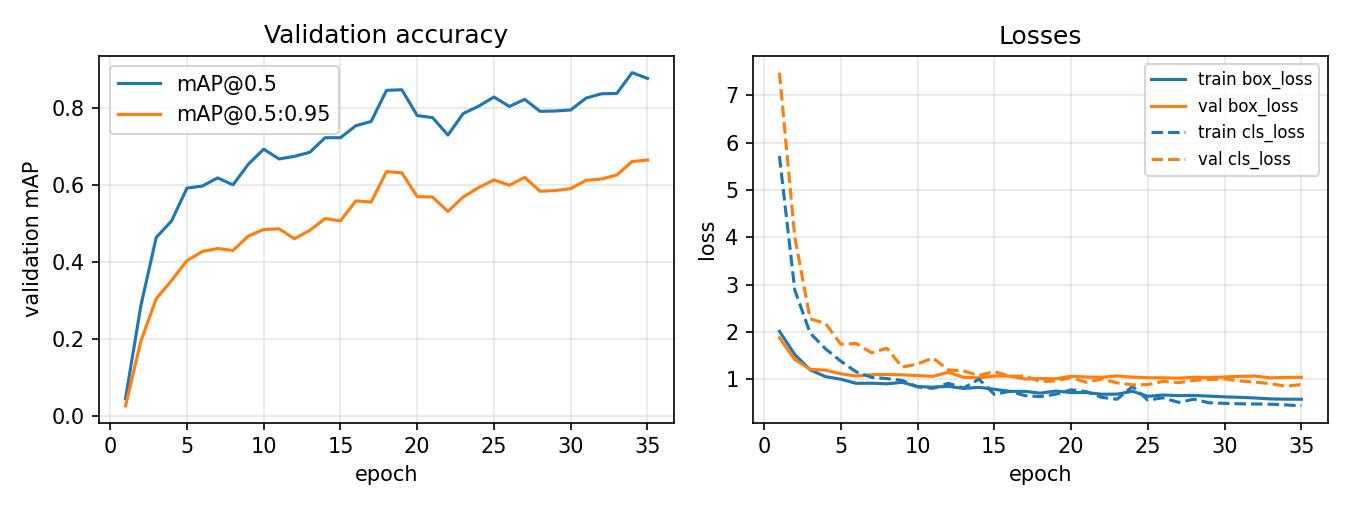
\includegraphics[width=\linewidth]{yolov8s_v2_training_curves.png}
\caption{Validation mAP and losses during fine-tuning (log stored in the selected checkpoint, epochs 1--35).}
\label{fig:curves}
\end{figure}

\section{Experiments}
\subsection{Detection accuracy}
Table~\ref{tab:det} reports the Ultralytics validator metrics. The test split, never used for training or
model selection, gives 0.893 mAP@0.5. Per class (test, AP@0.5), characters and objects with a clear outline
are near-perfect (\texttt{ally}, \texttt{player}, \texttt{crate}, \texttt{generateur}: 0.995), while bushes
are the weak point (0.515 on test, 0.611 on validation): they are large, irregular and merge into each other,
so box boundaries are ambiguous even for the annotator.

\begin{table}[t]
\centering\small
\setlength{\tabcolsep}{4pt}
\begin{tabular}{lrrrrr}
\toprule
Split & Img. & mAP@.5 & mAP@.5:.95 & P & R\\
\midrule
Val. & 19 & 0.876 & 0.668 & 0.812 & 0.812\\
Test & 9 & \textbf{0.893} & \textbf{0.701} & 0.846 & 0.843\\
\bottomrule
\end{tabular}
\caption{YOLOv8s at 800\,px (P: precision, R: recall). Validation was used for model selection.}
\label{tab:det}
\end{table}

\subsection{Input resolution}
The same model is evaluated at five input sizes (Table~\ref{tab:res}, Fig.~\ref{fig:res}). Latency is the
median wall-clock time of one \texttt{predict} call on a $1920\times1080$ frame (pre-processing, inference
and NMS) at batch size~1 in FP32, on a laptop RTX 3060 GPU and on an Intel Core i7-11800H CPU.
Accuracy peaks around the training resolution (800--1024\,px) and decreases slightly at 1280\,px. The cost of
resolution, however, depends on the hardware. On the GPU, latency barely changes between 480 and 800\,px
(10.6 and 11.5\,ms), consistent with a GPU under-used by single small images: the training resolution is
free and runs at 87 frames per second. On the CPU, latency grows roughly with the pixel count, and 480\,px
halves it at the cost of about 5 points of mAP@0.5:0.95. With nine test images, accuracy differences below
$\pm0.02$ should be read as noise.

\begin{table}[t]
\centering\small
\begin{tabular}{rrrrr}
\toprule
Input & mAP@.5 & mAP@.5:.95 & GPU & CPU\\
\midrule
480 & 0.854 & 0.649 & 10.6 ms & 95 ms\\
640 & 0.843 & 0.662 & 10.8 ms & 140 ms\\
800 & 0.893 & 0.701 & 11.5 ms & 212 ms\\
1024 & 0.905 & 0.703 & 15.5 ms & 304 ms\\
1280 & 0.897 & 0.687 & 22.1 ms & 470 ms\\
\bottomrule
\end{tabular}
\caption{Accuracy (test split) and median latency per 1080p frame versus input size (GPU: RTX 3060 Laptop;
CPU: i7-11800H).}
\label{tab:res}
\end{table}

\begin{figure}[t]
\centering
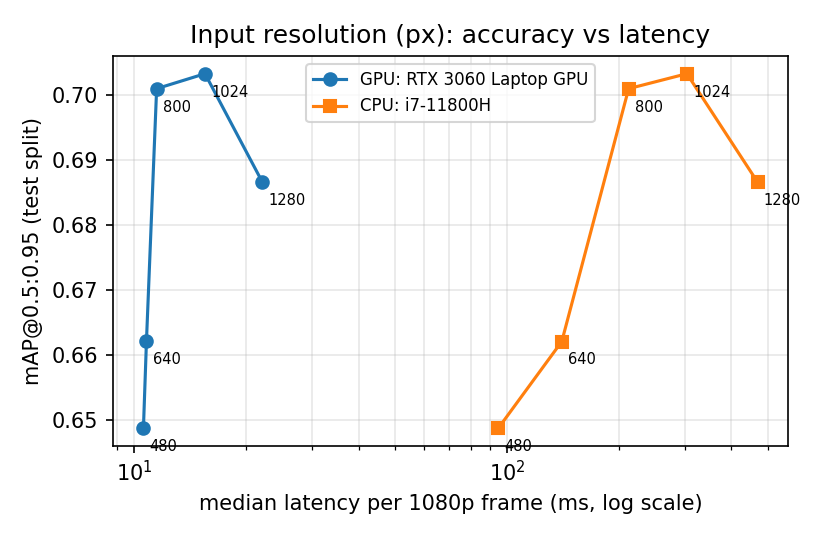
\includegraphics[width=\linewidth]{resolution_tradeoff_test_cpu_gpu.png}
\caption{Accuracy versus latency (log scale) for five input sizes on GPU and CPU.}
\label{fig:res}
\end{figure}

\subsection{Where do the errors come from?}
The detector's confusion matrix (validation, confidence 0.25, IoU 0.45) contains almost no confusion between
classes: only 2 of the 153 boxes (one ally and one enemy) receive the wrong label. Its errors are against the
background, and bushes dominate them: 14 of the 40 bushes are missed and 20 predicted bush boxes match no
annotation. The crop classifier isolates recognition from localisation by receiving the annotated box
(Table~\ref{tab:crop}). The ResNet-18 labels 95.4\% of the test crops correctly and \emph{every} bush (40/40
on validation, 23/23 on test). Bushes are therefore easy to recognise but hard to delimit: they form large
clusters whose split into boxes is ambiguous, which points to stricter annotation rules rather than a larger
model. The classifier's remaining errors are among characters (3 of its 4 test errors: player, ally and
enemy look alike and differ mostly by team markers; Fig.~\ref{fig:crop}). ImageNet pre-training mainly
accelerates convergence (validation macro-F1 0.96 after 10 epochs, against 0.69 from scratch); the final
scores differ by about one point, within noise for 87 test crops.

\begin{table}[t]
\centering\small
\begin{tabular}{lcc}
\toprule
Classifier & Val acc. / F1 & Test acc. / F1\\
\midrule
ResNet-18 (ImageNet) & 0.980 / 0.983 & \textbf{0.954} / \textbf{0.958}\\
Small CNN (scratch) & 0.967 / 0.972 & 0.931 / 0.948\\
\bottomrule
\end{tabular}
\caption{Crop classification of the annotated boxes (accuracy and macro-F1).}
\label{tab:crop}
\end{table}

\begin{figure}[t]
\centering
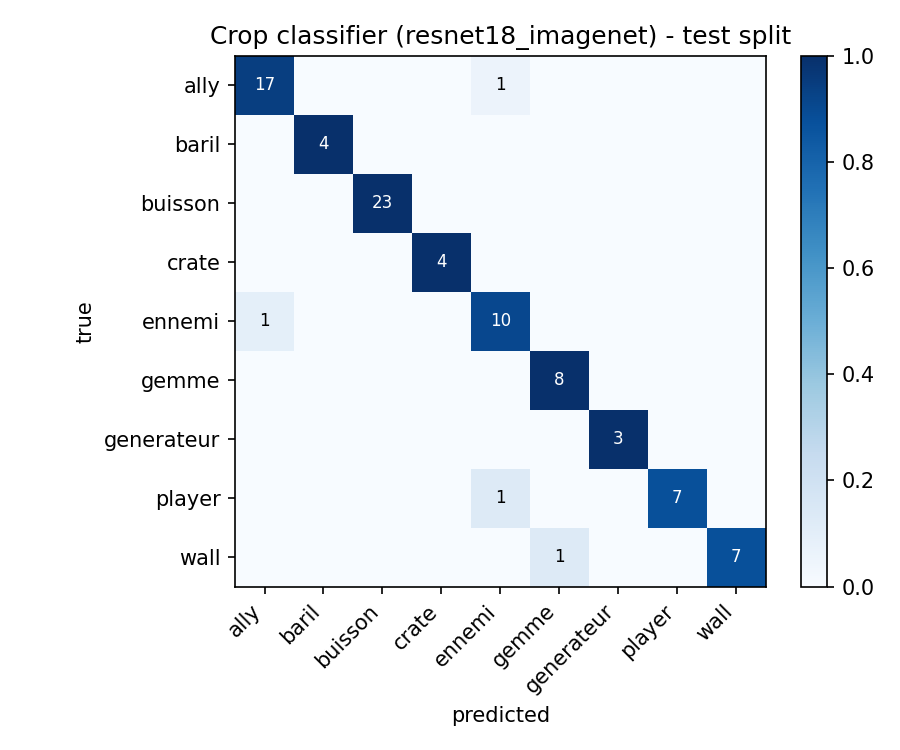
\includegraphics[width=0.9\linewidth]{resnet18_imagenet_confusion_test.png}
\caption{Confusion matrix of the ResNet-18 crop classifier on the test crops.}
\label{fig:crop}
\end{figure}

\section{Limitations}
The evaluation sets are small (19 and 9 images), so every score carries several points of uncertainty, and the
validation score is optimistic because the same split selected the checkpoint. The interface classes are not
evaluated, and all frames come from a few sessions: generalisation to other maps and modes is untested.

\section{Conclusion and future work}
Fewer than one hundred annotated frames are enough for a COCO-pretrained YOLOv8s to detect the main in-game
objects reliably and in real time; the remaining errors concentrate on amorphous classes such as bushes.
Next steps are to annotate more frames (bushes, interface screens) and report confidence intervals, to compare
model sizes and YOLOv9~\cite{wang2024yolov9} under the same protocol, and to measure the gain of an
ONNX/TensorRT export on GPU latency.

\bibliographystyle{plain}
\bibliography{references}
\end{document}
